\chapter{StockTwits Classified Sentiment and Stock Returns}

\section{Introduction}
\label{S:3.1}

Can the stock market be predicted by analyzing social media? Recent developments in machine learning and the growing quantities of available text data from online news, social media and annual reports have triggered intensive research in finance. In their pioneering paper, \citet{antweiler2004all} compute a bullishness measure out of 1.5 million messages posted on Yahoo! Finance and Raging Bull and find that stock messages help predict market volatility. Their results clearly reject the hypothesis that all that talk is just noise. They show that there is financially relevant information present in social media. In a similar vein, \citet{tet_07} constructs a measure of media pessimism from a Wall Street Journal column and finds that it predicts downward pressure on market prices. 

Most of the previous financial studies of social media rely on pre-defined or manually annotated sentiment dictionaries. Such approaches are limited in various ways. How to create a sentiment classifier that understands the vocabulary of the messages posted by the investors? For instance, ``bull" is an animal in everyday language but refers to someone optimistic in the financial jargon. \citet{loughran2011liability} create a words list, which helps classify tone in a financial document. However, this might not be sufficient in the context of social media because messages posted present many typos, abbreviations and slang, so one needs to have an additional layer of data preprocessing. For instance, the word ``goooooood" would not be recognized by the model if it is not corrected into ``good" first. On the other hand, manually annotating and validating dictionaries is not a scalable approach to handling social media content.

This chapter overcomes these limitations. We develop a machine learning algorithm to classify the sentiment of a large sample of StockTwits messages as bullish, bearish, or neutral. The sample consists of all messages referring to US and Canadian stocks, including ETFs and other types of securities available on CRSP/Compustat, from January 2010 to March 2020. We train our machine learning classifier on the set of all user sentiment-labeled messages, which constitute about one third of the sample. We then classify the sentiment of all remaining messages. Our method scales and performs very well. It achieves an out-of-sample accuracy of 85.9\%, which compares well to the anecdotal 80 to 85\% probability that human annotators agree on the sentiment of a document (see, e.g., \citet{wilson2005recognizing} and \citet{chen2020large}). As a side product, we generate a vocabulary of one million investor sentiment-labeled terms consisting of up to three words that frequently appear in StockTwits messages.

We then construct a stock-aggregate daily sentiment polarity measure and relate it to daily stock returns. We find that polarity is positively associated with contemporaneous returns. However, unconditionally, polarity cannot predict next-day returns, which is in line with the efficient market hypothesis (EMH). We then conduct an event study. We define events as days of sudden peaks of message volume of individual tickers. We classify events as bullish, bearish, or neutral depending on the prevailing polarities. We find that bullish (bearish) events are strongly associated with large positive (negative) abnormal returns. Cumulative abnormal returns over the preceding 20 days of an event have no predictive power on the type of event. Returns normalize immediately after the jump on the event date, which again is in line with the EMH. In contrast, remarkably, we find that cumulative abnormal polarity has statistically significant predictive power on the type of event. We assess the economic relevance of our findings with the performance of cumulative abnormal polarity ranked portfolios. We find that for appropriate choices of thresholds, cumulative abnormal polarities provide valuable signals for stock market investments.

As a technical byproduct, we develop a sentiment classifier of micro-blogs for imbalanced data. This addresses the stylized fact that bloggers post more bullish than bearish-labeled messages. In our sample, the ratio is five to one. On the other hand, we find that not all messages carry a substantial stock market relevant sentiment. Rather than re-sampling from the underrepresented bearish class, we thus introduce an auxiliary neutral class. We then run two independent binary classifiers. The first (second) classifies messages as bullish versus non-bullish (bearish versus non-bearish). We aggregate the two binary outcomes and classify a message as bullish (bearish) for the concordant combination bullish/non-bearish (non-bullish/bearish), and neutral otherwise. This approach is very simple and efficient, and eliminates the class imbalance bias at the same time. It builds on any traditional binary classifier. We use logistic regression on Term Frequency-Inverse Document Frequency (TFIDF)-vectorized messages. TFIDF is a weighting scheme gauging the importance of a word in a document.

This chapter contributes to the growing literature on machine learning classification of social media and its interaction with the stock market. Most previous financial studies use Twitter as their primary source of data. Twitter has the advantage of being used by a wide range of people across the world and a few influencers can attract the attention of many investors. In 2013, following a meeting with Tim Cook (Apple CEO), Carl Icahn tweeted that he bought a large position in Apple and believed that the company is extremely undervalued. This bullish tweet caused the market capitalization of Apple to jump by \$12 billion. In 2019, JPMorgan has created the Volfefe Index to track Donald Trump's tweets impact on the stock market. However, it is more difficult to disentangle noise from relevant tweets in Twitter than in other more focused social media. Results from \citet{Ghoshal} show that StockTwits is significantly more informative than Twitter data. This is not surprising as StockTwits is a finance-focused platform whereas Twitter also captures irrelevant opinions on a wide range of non-finance related matters. 

This chapter is the first work that analyzes the predictive power of StockTwits messages on stock returns unconditionally and around specific events. \citet{renault2017intraday} builds an intraday investor sentiment indicator using messages and finds that the change in investor sentiment of the first half-hour of a trading day helps forecast the last half-hour market return of that trading day. However, his classifier is based on a dictionary consisting of 8 thousand manually validated and modified terms, which limits its scalability. \citet{renault2020sentiment} uses larger data sets and compares various classifiers, including machine learning. 

Our approach is in some parts similar to \citet{ranco2015effects}, who also study the relation of micro-blog sentiments with stock returns. However, they use Twitter data, whereas the finance-tailored StockTwits data we use results in higher contemporaneous correlations between stock returns and polarity. They manually annotate 100 thousand tweets, which limits the scalability of their approach. Our sample is much larger (90 million versus 1 million messages) and covers a longer period (10 years versus 13 months). 

\citet{ke_kel_xiu_20} extract sentiment from news articles on the Dow Jones Newswires. They train a  sentiment score directly on returns. In contrast, we use user sentiment-labeled StockTwits messages as the training and validation set for our sentiment classifier.


This chapter also contributes to the EMH literature by gauging how cumulative average abnormal returns and abnormal polarities behave around sudden peaks of message activity. 



The remainder of the chapter is structured as follows. Section \ref{S:data} discusses StockTwits and stock market data. Section \ref{S:classification} develops our sentiment classifier based on TFIDF vectorization. Section \ref{S:polarity} introduces the sentiment polarity measure and relates it to stock returns. Section \ref{S:event studies} contains the event study. Section \ref{S:portfolios} discusses the sentiment-sorted portfolio performance. Section \ref{S:conclusion} concludes. The appendix contains additional statistics and background material.


\section{StockTwits and Stock Market Data}
\label{S:data}

StockTwits is a large social media platform similar to Twitter but designed for investors and traders. Users register online and can post messages about any listed stock through the prefix \$ followed by the ticker of the stock. StockTwits was created in 2008 as an app built on the Twitter's API and later detached from Twitter to build a standalone social network. As of April 2019, it had over two million registered users and the number of daily posted messages has been growing exponentially, see Figure~\ref{fig:tweet_vol_daily}. 

\clearpage 

\begin{figure}[h]
    \centering
    \includegraphics[width=0.75\textwidth]{tweet_vol_daily.JPG}
    \mycaption{Number of messages posted daily on StockTwits}{Message volume posted on StockTwits. Numbers are aggregated daily.}
    \label{fig:tweet_vol_daily}
\end{figure}


StockTwits describes itself as ``the voice of social finance and the best way to find out what is happening right now in the markets and stocks you care about''. In practice, it is effectively used by finance professionals to express their opinions on individual stocks and the market as a whole. Importantly, users have the option to label their posted messages as either bullish or bearish.\footnote{This optional label was effectively available as of mid-2010.} This feature is key for our approach, as it allows for sentiment classification of all messages using machine learning trained on the user-labeled messages.\footnote{One third of the messages in our sample have a user labeled sentiment.} 

The reasons for using StockTwits and not other social media data for financial studies are at least threefold. First, a major challenge in applying natural language processing is the creation of an appropriate labeled vocabulary. \citet{loughran2011barron} show that it is essential to have a specific vocabulary to interpret finance documents (i.e., many words have a different meaning in finance than in traditional English, such as “bear trap”). In addition to that, social media slang is an additional layer of language complexity. To this extent, the functionality to self-tag bullish and bearish messages on StockTwits is extremely valuable as it allows the creation of a specific labeled vocabulary out of labeled messages. We are not aware of any other social media platform in finance offering this functionality. Second, text data from StockTwits is more reliable and less noisy than from general purpose platforms, such as Twitter, because messages focus on finance and economics matters only. Micro-bloggers have incentives to post valuable information in order to maintain or increase mentions and retweets, and thus have a greater share of voice in the forum (\citet{sprenger2014tweets}). On the other hand, StockTwits messages might be biased and subject to malicious users that try to manipulate the market. However, market manipulations likely happen only rarely as the SEC closely monitors potential influencers to prevent any market abuse. Third, extracting data from StockTwits is easy because of its API. StockTwits' API is designed to query the database to download messages via JSON requests. We provide a short tutorial in Appendix~\ref{app_tut}.

We use stock market data from CRSP/Compustat. We extract daily closing prices, daily volume of transactions and number of shares outstanding for all US and Canadian stocks, as well as ETFs and some other types of securities, from January 2010 to March 2020. Stock prices and number of shares are adjusted to account for any distribution (i.e., dividends, stock splits) so that a comparison can be made on an equivalent basis before and after the distribution. We use as risk-free rate the 3-month US T-bill rate, converted into daily risk-free returns. We henceforth refer to daily stock excess returns over risk-free simply as returns. Using a Python script, we then extract all messages from StockTwits for the list of tickers corresponding to the sample of US and Canadian stocks. This results in 90 million messages, which we download and store as JSON files.\footnote{A message may refer to multiple tickers. We count any such message towards any ticker that it refers to. We give more information about this double counting in Appendix \ref{app_counting}.} Overall, our sample covers 8843 tickers, whereof 75\% refer to ordinary common share, 15\% to ETFs, and the remaining 10\% to other types of securities. Henceforth, we interchangeably refer to any of these securities as either a stock or a ticker. 

Every StockTwits message includes eight features: (1) the reference ticker(s), (2) a timestamp, (3) a unique message identifier, (4) the body of the message, (5) the sentiment label (bearish, bullish, or none) entered by the user, (6) a unique identifier of the user who posted the message, (7) the number of messages published by the user who posted the message, and (8) the number of followers of the user who posted the message. Our sentiment analysis builds on the first five features. The last three provide additional information on the network structure, which we briefly discuss in Appendix \ref{app_userstats}.

Figure~\ref{screenshot} shows a screenshot of the StockTwits website as of 3rd March 2020, for a query of AAPL, which is the ticker for Apple. The first message is labeled as bullish by the user ``satkaru", the two next are unlabeled messages that will be classified by our machine learning algorithm, and the last message is labeled as bearish by the user ``Etrading''. 

\begin{figure}[h]
\centering
\includegraphics[width=0.75\textwidth]{stocktwits_screeshot_3march2020.JPG}
\mycaption{Screenshot of messages posted on StockTwits}{Screenshot is from the 3rd of March 2020 for a query on AAPL, the ticker of Apple.}
\label{screenshot}
\end{figure}


The left plot of Figure \ref{fig:data-stocktwits2} shows the top 30 most discussed tickers on StockTwits. SPY, a large ETF that tracks the S\&P 500 stock market index, is the most discussed ticker, followed by Apple and other big tickers. The messages about the 15 (30) biggest tickers represent 20\% (25\%) of the total number of messages, which indicates that users talk about a wide panel of tickers and not only big firms. The right graph shows a histogram of the number of messages per ticker. The x-axis is log-scaled because due to extreme values the distribution is highly skewed. 

\begin{figure*}[h]
\centering
\begin{subfigure}{0.49\textwidth}  
            \centering 
            \includegraphics[width=\textwidth]{top30tickers.jpg}
        \end{subfigure}
        \begin{subfigure}{0.49\textwidth}   
            \centering 
            \includegraphics[width=\textwidth]{LogTweetsPerFirm_3.jpg}
        \end{subfigure}
        \mycaption{Ticker summary statistics}{
        Left graph shows the top 30 most discussed tickers on StockTwits. SPY is the ticker of a large ETF tracking the S\&P 500 and AAPL is the ticker for Apple. Right graph shows the distribution of the number of messages across tickers.} 
        \label{fig:data-stocktwits2}
\end{figure*}


Text messages need to be transformed into a quantitative vector to be fed into our machine learning classifier, which in turn computes a sentiment score. This transformation consists of several steps. First, we apply some preprocessing operations to the text messages: an apostrophe handler, a contraction form handler (e.g., ``aren't" becomes ``are not"), tickers removal, stop words removal (e.g., ``a", ``the", ``of")\footnote{We follow \citet{renault2020sentiment} and \citet{saif2014stopwords} and use a restrictive list of stopwords to avoid accuracy decrease.}, users removal, lemmatization, URLs removal and a simple spell corrector dealing with more than two repeated characters (e.g., ``soooo goooood" becomes ``soo good"). Table \ref{tab:preprocess} shows five examples of messages before and after preprocessing.


\begin{table}[h]
\centering
\begin{tabular}{ll} \hline
\multicolumn{2}{l}{Before preprocessing}                                   \\ \hline  
(1) & @CassandraTwit \$uvxy contango 3.5\%...still long. goooooood        \\
(2) & \$FRPT Take profits while you still can.                            \\
(3) & \$UVXY \$tvix go time boys and girls. Holding overnight again       \\
(4) & \$dnr Nice upgrade as company goes into its quiet period!           \\
(5) & \$SPY market won't reverse again towards closing. Get put options.  \\ \hline   \hline
\multicolumn{2}{l}{After preprocessing}                                   \\ \hline 
(1) & contango still long good                                            \\
(2) & take profit while you still can                                     \\
(3) & go time boy and girl hold overnight again                           \\
(4) & nice upgrade as company go into its quiet period                    \\
(5) & market will not reverse again towards closing get put options      \\ \hline
\end{tabular}
\mycaption{Preprocessing of five sample messages}{Preprocessing operations include: punctuation removal, lower casing, apostrophe handling, contraction form handling (i.e., ``won't" becomes ``will not"), tickers removal, users removal, URLs removal, parsing and a simple spell corrector dealing with more than two repeated characters (i.e., ``goooood" becomes ``good")}
\label{tab:preprocess}
\end{table}


The next step is tokenization: the slicing of a text message into smaller units called terms or tokens. In financial lingo, some words only have meaning when associated with other words (i.e., ``bad apple" or ``bear flag"). $N$-gram models allow accounting for words frequently occurring together with other words. The main hyperparameter in an $N$-gram model is the number $N$ of words that form a term: a unigram is a term with only one word, a bigram is a term with two consecutive words, etc. Larger $N$-gram models increase dramatically the size of the vocabulary (i.e., the collection of all terms considered). We select $N=1,2,3$ and truncate the resulting vocabulary such that it consists of the one million most frequent terms in the union of all unigrams, bigrams and trigrams. 

\begin{figure}[h]
\centering
\begin{subfigure}{0.49\textwidth}
\centering
\includegraphics[width=1\textwidth]{Positive rate words.jpg}
\end{subfigure}
\begin{subfigure}{0.49\textwidth}
\centering
        \includegraphics[width=1\textwidth]{Negative rate words.jpg}
\end{subfigure}
    \mycaption{Word clouds}{Bullish word cloud (left), bearish word cloud (right). These correspond to the most frequent terms (up to trigrams) in user-labeled bullish (bearish) messages relative to their total appearance. The size of the terms represents their importance in the cloud.}
    \label{wordclouds}
\end{figure}


Figure \ref{wordclouds} represents the bullish and bearish word clouds. These represent the most frequent terms in all user-labeled bullish and bearish messages relative to their total appearance, respectively. The size of the terms represents their relative weight in the cloud. In the bullish cloud, we see terms such as ``bullish divergence", ``room to grow", ``lot potential" which we can clearly interpret as bullish signals. In the bearish cloud, we find terms such as ``recent resistance", ``short setup", ``bad apple" which again we can directly interpret as bearish signals. These findings are reassuring in the sense that the content of the messages on StockTwits are consistent with their labels. We checked for anomalies at random, but did not find significant issues. Appendix \ref{app_ano} discusses two such anomalies. 






%\begin{figure}[h]
%\begin{center}
%    \includegraphics[width=0.5\textwidth]{Positive rate words.jpg}

%    \vspace{1cm}

%    \includegraphics[width=0.5\textwidth]{Negative rate words.jpg}
%   \vspace{0.1cm}
%    \caption{Bullish word cloud (top), bearish word cloud (bottom). These correspond to the most frequent terms (up to trigrams) in user-labeled bullish (bearish) messages relative to their total appearance. The size of the terms represent their importance in the cloud.}
%    \label{wordclouds}
%  \end{center}
%\end{figure}


\section{Sentiment Classification}\label{S:classification}

The left plot of Figure \ref{fig:classif_time} shows the proportions of user sentiment-labeled messages across time. In the early years of the platform, most messages were unlabeled, presumably because users were not familiar with the sentiment label yet. Albeit the proportion of unlabeled messages monotonically declines over the years, almost 60\% of the more recent messages are still unlabeled. Overall, around 30 million messages are user-labeled and 60 million messages are unlabeled. We conjecture that by far not all unlabeled messages reflect market neutral opinions. Indeed, the right plot of Figure \ref{fig:classif_time} reveals that a substantial part of user-unlabeled messages is machine learning classified as bullish or bearish. Hence these user-unlabeled messages contain indeed market relevant information, which we are able to capture by our algorithm. 

%\begin{figure}[h]
%    \centering
%    \includegraphics[width=0.5\textwidth]{preclassif_acrosstime.JPG}
%    \caption{Proportions of user-labeled messages: bullish (green), bearish (red), and unlabeled (gray) across time. Proportions are aggregated monthly.}
%    \label{fig:ts_neutral_vs_uncl}
%\end{figure}

\begin{figure}[h]
\centering
\begin{subfigure}{0.49\textwidth}
\centering
\includegraphics[width=1\textwidth]{preclassif_acrosstime.JPG}
\end{subfigure}
\begin{subfigure}{0.49\textwidth}
\centering
        \includegraphics[width=1\textwidth]{postclassif_acrosstime3.JPG}
\end{subfigure}


    \mycaption{Message classification}{Left plot shows the proportions of user-labeled messages: bullish (green), bearish (red), and unlabeled (gray) across time. The right plot shows the proportions of machine learning classified messages: bullish (light green predicted, green user-labeled), bearish (light red predicted, red user-labeled), and neutral (gray) across time. Proportions are aggregated monthly.}
    \label{fig:classif_time}

\end{figure}

Among the user-labeled messages we find five times more bullish than bearish ones. This ratio indicates that investors are on average optimistic about the market, which is consistent with findings in the literature, e.g., \citet{renault2017intraday}. Such an imbalance is a well-known issue in machine learning classification as it creates a bias towards the over-represented class (see \citet{chawla2004special}). There are various ways to tackle class imbalance. An all-purpose standard approach in machine learning is to over-sample the minority class, which consists of randomly re-sampling from the minority class and thus artificially re-balance the class sizes in the data. We use a different approach, which is tailored for our setup. As not every message carries a substantial stock market relevant sentiment, we deviate from the bullish--bearish dichotomy. Instead, we create an auxiliary neutral sentiment class to account for messages that do not take a clear stand. See Appendix \ref{app_exampleclass} for examples of such neutral messages.

We then run two independent binary classifiers. The first (second) classifies messages as bullish versus non-bullish (bearish versus non-bearish). We aggregate the two binary outcomes and classify a message as bullish (bearish) for the concordant combination bullish/non-bearish (non-bullish/bearish), and neutral otherwise. This approach is very simple and efficient, and eliminates the class imbalance bias at the same time. It builds on any traditional binary classifiers. We use logistic regression on Term Frequency-Inverse Document Frequency (TFIDF)-vectorized messages, as in, e.g., \citet{nlp1}, \citet{classifq}, \citet{erdemlioglu2017market}. TFIDF is a widely used method to transform a text, in our case a message $m$, into a numerical vector, $TFIDF_m$. The dimension of this vector is equal to the size of the vocabulary (the collection of all terms across all messages). The components of the vector encode the importance of the corresponding terms $t$ in the message $m$, as formally defined by $TFIDF_{m,t} = TF_{m,t} \cdot IDF_t$. The first factor measures how frequently term $t$ appears in the message,
\begin{equation}
TF_{m,t} =\dfrac{\sum_{i=1}^{N_m} \textbf{1}_{t=t_{m,i}}}{N_m},
\end{equation}
where $N_m$ denotes the number of terms $t_{m,i}$ in message $m$. The second factor measures how important term $t$ is to the message,
\begin{equation}
IDF_t = \log \big(\dfrac{V}{\sum_{j=1}^{V} \textbf{1}_{t \in m_j}}\big),
\end{equation}
where $V$ denotes the total number of messages $m_j$. A term $t$ appearing in many documents (such as ``the", ``is", ``of") is likely to have low information content, hence a low $IDF_t$. 

We use 80\% of the user sentiment-labeled messages as a training set and keep 20\% as a test set, then we run two binary classifiers. The first (second) classifier sets bullish (bearish) as positive and non-bullish (non-bearish) as negative class. Every message then classifies into one of the following combinations: (non-bullish, bearish), (bullish, bearish), (non-bullish, non-bearish), (bullish, non-bearish). For the first and last combinations, the two algorithms agree and the final classification is defined to be bearish (non-bullish, bearish) or bullish (bullish, non-bearish), respectively. For the two middle combinations, (bullish, bearish) and (non-bullish, non-bearish), the two algorithms disagree, so that the final classification is defined to be neutral. Formally, every message $m$ is mapped onto either
\begin{equation}
     m\mapsto \begin{cases} \text{(non-bullish, bearish)} & =: \text{bearish} \\ \text{(bullish, bearish)}& =: \text{neutral} \\ \text{(non-bullish, non-bearish)}& =: \text{neutral} \\ \text{(bullish, non-bearish)} &=: \text{bullish.} \end{cases}
\end{equation}

To select optimal classification thresholds, we maximize the F1 scores. The F1 scores of the two binary classifiers differ because they depend on which class is defined as the positive one. We recap the definition of the F1 score in Appendix \ref{app_class}. Figure~\ref{fig:optimal_thresholds} shows the F1 scores as functions of the threshold. Circles indicate the maximal F1 scores, along with the corresponding optimal thresholds, 0.50 and 0.72, respectively. 

\begin{figure}[h]
    \centering
    \includegraphics[width=0.75\textwidth]{optimal thresholds.JPG}
    \mycaption{Optimal classification thresholds}{The green (red) line is the F1 score for the bullish versus non-bullish (bearish versus non-bearish) classifier as a function of the threshold. Circles indicate the maximal F1 scores.}
    \label{fig:optimal_thresholds}
\end{figure}

If the sentiment score of a message is bigger (smaller) than 0.72 (0.50), respectively, then both classifiers agree and the sentiment of the message is classified as bullish (bearish), respectively. If the sentiment score is between 0.50 and 0.72, the classifiers disagree, (bullish, bearish), and we consider the message as neutral. Finally, we overwrite the predicted sentiment of any message by the user-labeled sentiment whenever the latter is available. Research in sentiment classification shows that human annotators tend to agree about 80 to 85\% of the time when evaluating the sentiment of a document (see, e.g., \citet{wilson2005recognizing} and \citet{chen2020large}). This is a benchmark for the accuracy that a sentiment classifier should meet or beat. The out-of-sample accuracy of our combined classifier is 85.9\%. Appendix~\ref{app_class} provides in-sample and out-of-sample confusion matrices for our combined classifier.

The right plot of Figure \ref{fig:classif_time} shows the proportions of our machine learning classifications across time. Percentages of bearish (user-labeled and classified as bearish) and bullish (user-labeled and classified as bearish) messages are stable over time, suggesting that our classification method is robust. Even if most messages were not user-labeled in the early years of the platform, as seen in the left plot of Figure \ref{fig:classif_time}, we are now able to classify the sentiment of all messages in the sample, including a neutral class. Consistent with the over-representation of bullish messages observed in the user-labeled messages, there are substantially more messages classified as bullish than bearish. Examples of classified messages are given in Appendix \ref{app_exampleclass}.

%\begin{figure}[h]
%    \centering
%    \includegraphics[width=0.5\textwidth]{postclassif_acrosstime3.JPG}
%    \caption{Proportions of machine learning classified messages: bullish (light green predicted, green user-labeled), bearish (light red predicted, red user-labeled), and neutral (gray) across time. Proportions are aggregated monthly.}
%    \label{fig:postclassif_acrosstime}
%\end{figure}






%\clearpage
\section{Polarity}\label{S:polarity}

We next aggregate message sentiments on a daily ticker-level and across the market. Thereto, we denote $C_{i,t,j}=1,0,-1$ for bullish, neutral, bearish, respectively, the sentiment of the $j$th message about ticker $i$ on day $t$.\footnote{We follow the close-to-close convention. First, we remove all non-business days from the sample, whereby messages posted on non-business days count towards the next business day. ``Day $t$'' then stands for the time interval from 4pm on the previous business day $t-1$ to 4pm on business day $t$. This convention is consistent with the stock return data, which are close-to-close, and thus avoids any look-ahead bias of our sentiment polarity.} We follow \citet{ranco2015effects} and define the sentiment polarity of ticker $i$ on day $t$ as
\begin{equation}
    P_{i,t} = \dfrac{\sum_{j=1}^{V_{i,t}} (\textbf{1}_{C_{i,t,j} = 1} - \textbf{1}_{C_{i,t,j} = -1})}{\sum_{j=1}^{V_{i,t}} (\textbf{1}_{C_{i,t,j} = 1} + \textbf{1}_{C_{i,t,j} = -1})},
\end{equation}
where $V_{i,t}$ denotes the number of messages about ticker $i$ on day $t$.\footnote{If $V_{i,t}=0$ then we set $P_{i,t} =0$.} 

As an aggregate, we define the market polarity as a weighted average over all tickers 
\begin{equation}
\label{marketpoleq}
    P_t^M = \dfrac{\sum_{i} V_{i,t} \cdot P_{i,t}}{V^M_t} ,
\end{equation}
where $V^M_t = \sum_{i} V_{i,t}$ denotes the number of messages on day $t$. Figure \ref{fig:marketpolspy} shows a scatter plot of the market polarity $P_{t}^M$ versus the polarity of SPY. The slope coefficient of the regression line is statistically significantly positive and the contemporaneous Pearson correlation coefficient is 0.53, suggesting that the market polarity is an accurate measure of the aggregated sentiment of the market.\footnote{We do not expect $P^M_t$ to be equal to the SPY polarity because the underlying sets of stocks differ: market polarity contains stocks that are not in the S\&P500 and vice versa.} Also, consistent with Figure \ref{fig:classif_time}, SPY and market polarities are bullish-biased.

\begin{figure}[h]
    \centering
    \includegraphics[width=0.75\textwidth]{spy_vs_marketpol.JPG}
    \mycaption{Market polarity versus SPY polarity}{The red line shows the linear regression line and coefficients.}
    \label{fig:marketpolspy}
\end{figure}


For the following time series analysis and event study we restrict our sample. There are two reasons for doing so. First, we keep computational cost at a reasonable level. Second, and more importantly, the time series of ticker-individual polarities exhibit spikes and are too noisy if the daily message volumes $V_{i,t}$ are too small. We therefore exclude from now on tickers whose median of daily message volume is less than 50. Our reduced sample contains 19 tickers, covering a range of security types, sectors, and market capitalization. We refer to Appendix \ref{app_coverage} for more details on the coverage, including summary statistics and the list of tickers covered.

To understand how our polarity measure is related to investor sentiment, we run linear regressions of contemporaneous and next-day returns on polarity:
\begin{align}
    R_{i,t} &= \alpha^{cont} + \beta^{cont} \cdot P_{i,t} + \epsilon^{cont}_{i,t}, \\
    R_{i,t+1} &= \alpha^{next} + \beta^{next} \cdot P_{i,t} + \epsilon^{next}_{i,t}.
\end{align}
Table \ref{regpolret} shows that the regression coefficient is positive and significant for contemporaneous returns. This indicates that polarity is a good contemporaneous proxy for the sentiment of investors. Further supporting evidence is given by the correlation between polarity and contemporaneous returns at the ticker level. 

\begin{table}[h]
\centering
\begin{tabular}{l|c|c|c|c|c}
                     & $R_{i,t}$  & $R_{i,t+1}$        \\ \hline   
Constant             & -0.0047***  & -0.0002      \\
                     & (0.000)     & (0.000)      \\
$P_{i,t}$           & 0.009***      & 0.0003       \\
                     & (0.000)       & (0.000)      \\ \hline
$R^2$                & 0.012         & 0.000             \\
No. Obs.             & 34100         & 34100            
\end{tabular}
\mycaption{Regressions of returns on polarity}{Results from linear regressions of contemporaneous and next-day stock returns on polarity. Stock returns are trimmed at the 5\% percentile on both sides. Standard errors are reported in parentheses. Statistical significance at the 99\%, 95\%, and 90\% level is indicated with ***, **, *, respectively.}
\label{regpolret}
\end{table}


Figure \ref{fig:ts} shows the time series during 2019 for the top 6 most discussed tickers. In our entire sample of tickers, correlations are always positive and range between 0.1 and 0.3. In contrast, regressing next-day returns reveals that polarity has no predictive power for next-day stock returns unconditionally. In the following section we show how polarity has predictive power around specific events.

\begin{figure*}[h]
        \centering
        \begin{subfigure}[b]{0.425\textwidth}
            \centering
            \includegraphics[width=\textwidth]{ts_pol_ret_aapl.JPG}
        \end{subfigure}
        \quad
        \begin{subfigure}[b]{0.425\textwidth}  
            \centering 
            \includegraphics[width=\textwidth]{ts_pol_ret_amzn.JPG}
        \end{subfigure}
        \vskip\baselineskip
        \begin{subfigure}[b]{0.425\textwidth}   
            \centering 
            \includegraphics[width=\textwidth]{ts_pol_ret_tsla.JPG}
        \end{subfigure}
        \quad
        \begin{subfigure}[b]{0.425\textwidth}   
            \centering 
            \includegraphics[width=\textwidth]{ts_pol_ret_spy.JPG}
        \end{subfigure}
                \vskip\baselineskip
        \begin{subfigure}[b]{0.425\textwidth}   
            \centering 
            \includegraphics[width=\textwidth]{ts_pol_ret_amd.JPG}
        \end{subfigure}
        \quad
        \begin{subfigure}[b]{0.425\textwidth}   
            \centering 
            \includegraphics[width=\textwidth]{ts_pol_ret_fb.JPG}
        \end{subfigure}
        \mycaption{Correlation between return and polarity}{Time series of daily polarity (red - left axis) and daily stock returns (blue - right axis) since 1st of January 2019 for the top 6 most discussed tickers. Pearson correlation between the two time series is shown in the title.} 
        \label{fig:ts}
    \end{figure*}

\clearpage\section{Event Study}\label{S:event studies}

Event studies constitute a statistical method widely used in financial econometrics (see, e.g., \citet{mackinlay1997event}). In general, they are used to measure the effect of events on the market value of stocks. Well-known applications of event studies include the testing of various forms of the efficient market hypothesis (EMH) (see \citet{fama1969} and \citet{fama1991efficient}). 


\subsection{Events}
We define events as days with an unusual large number of messages for individual tickers. We conjecture that a sudden peak in StockTwits message volume indicates that an important corporate or stock market event is happening on the day of the peak. Figure \ref{fig:actvol} shows that increases (decreases) in message volumes are positively associated with increases (decreases) in contemporaneous weekly stock transaction volumes. These co-movements indicate that investors who post messages about stocks also trade them accordingly, adjusting their portfolios. This suggests that message volume peaks are a good proxy for corporate and stock market events.


\begin{figure}[h]
    \centering
    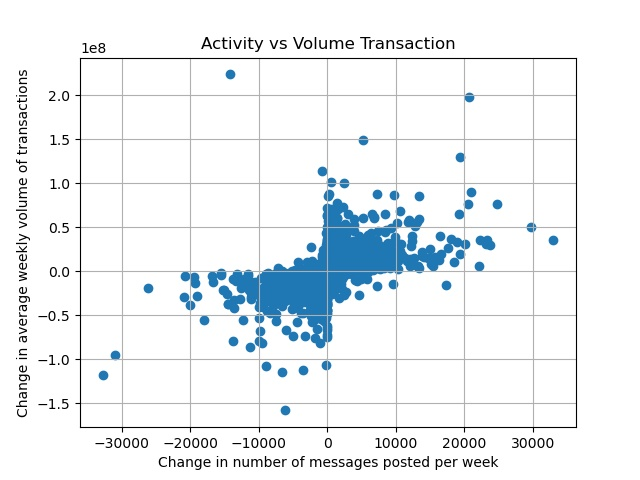
\includegraphics[width=0.75\textwidth]{activity-volume.jpg}
    \mycaption{Message activity and transaction volume}{Changes in weekly volume of transactions on the y-axis versus changes in message activity on the x-axis. Activity is measured in weekly messages posted per ticker.}
    \label{fig:actvol}
\end{figure}

\clearpage

To measure unusual activity peaks, we use as benchmark model a one-year rolling window regression of daily relative message volume changes of ticker $i$ on daily relative total message volume changes.\footnote{Accounting for the lead time of the one-year rolling estimation window, the event study effectively applies to the shorter period from January 2011 to March 2020.} Formally,
\begin{equation}
\dfrac{\Delta V_{i,t}}{V_{i,t-1}} = \alpha_i^V + \beta_i^V \cdot \dfrac{\Delta V_t^M}{V_{t-1}^M} + \epsilon_{i,t},    
\end{equation} 
which gives the one-year rolling estimates $\hat{\alpha}_i^V$ and $\hat{\beta}_i^V$. We then define the abnormal message volume changes for ticker $i$ on day $t$ as 
\begin{equation}
    AV_{i,t} = \dfrac{\Delta V_{i,t}}{V_{i,t-1}} - \left(\hat{\alpha}_i^V + \hat{\beta}_i^V \cdot \dfrac{\Delta V_t^M}{V_{t-1}^M}\right).
\end{equation}
We define an event for ticker $i$ as any day $t$ where the standardized abnormal volume exceeds two, 
\begin{equation}
    \dfrac{AV_{i,t} - \hat{\mu}_{AV_i}}{\hat{\sigma}_{AV_i}} > 2,
\end{equation}
where $\hat{\mu}_{AV_i}$ and $\hat{\sigma}_{AV_i}$ denote the one-year rolling empirical mean and standard deviation. 



Next we define the type of the event as either bullish, neutral or bearish. We use the abnormal polarity $AP_{i,t}$ of the event date to assess how on average investors perceive the event. Figure \ref{fig:abnpol_all} shows the distribution of abnormal polarities on event dates. 
\begin{figure}[h]
    \centering
    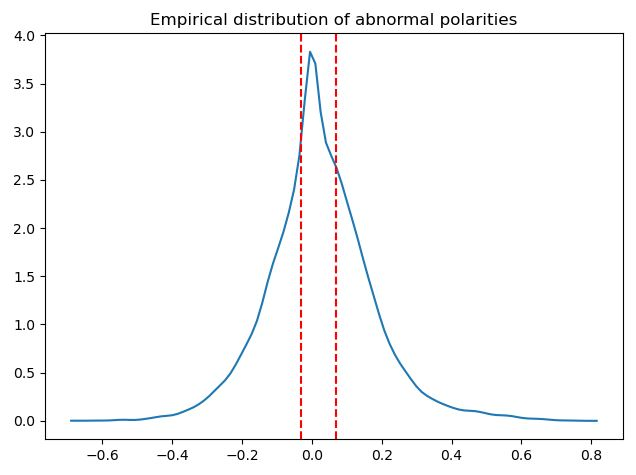
\includegraphics[width=0.75\textwidth]{abnpol_distr_all.JPG}
    \mycaption{Empirical distribution of abnormal polarities on event dates}{The red dashed lines show the one-third and two-third percentiles.}
    \label{fig:abnpol_all}
\end{figure}
We chose to use the one-third (-0.03) and two-third percentile (0.07) of the distribution of abnormal polarities as thresholds for the type of the event. We define the type of the event for ticker $i$ at $t$ as
\begin{equation}
Type_{i,t}= \begin{cases}
      Bullish  & \text{if}\ \ AP_{i,t}> 0.07, \\
      Neutral  & \text{if}\ \ AP_{i,t} \in [-0.03, 0.07], \\
      Bearish  & \text{if}\ \ AP_{i,t} < -0.03. \\
\end{cases}    
\end{equation}    

Overall, across 19 tickers, we identify 1131 events, whereof 454 bullish, 294 neutral, and 383 bearish types. This coverage is on par with previous studies (e.g., \citet{mackinlay1997event} analyze 30 stocks and 600 events). Figure \ref{fig:events} shows the aggregate events and their types across time. The count of events looks stationary over time, apart from a build up phase of the platform in the early part until 2014. The distribution of event types is also balanced across time.

\begin{figure}[h]
    \centering
    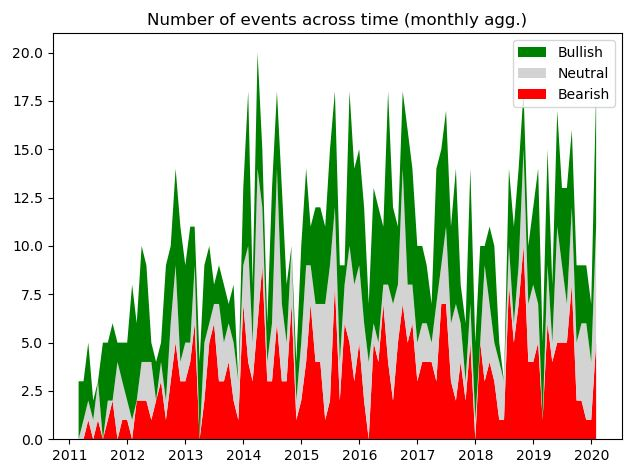
\includegraphics[width=0.75\textwidth]{events_across_time.JPG}
    \mycaption{Number of events of each type across time}{The green area shows bullish events, the gray area shows neutral events and the red area shows bearish events. Numbers are aggregated monthly.}
    \label{fig:events}
\end{figure}

As an illustration, Figure \ref{fig:activityaapl} shows for Apple the time series of message volume and the corresponding events. Between January 2011 and March 2020, our algorithm identified 73 events for Apple. 
\begin{figure}[h!]
    \centering
    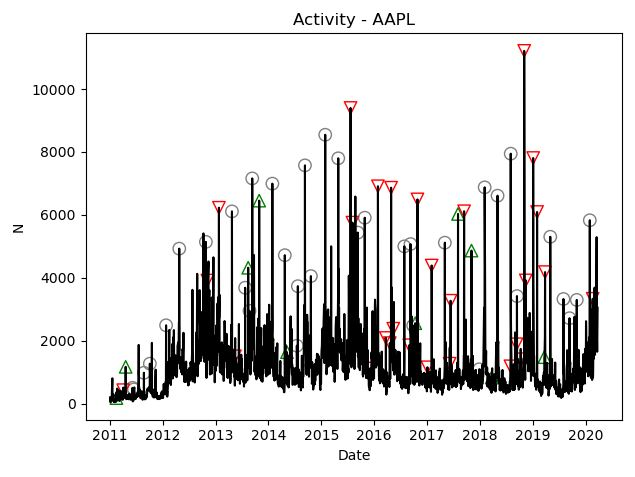
\includegraphics[width=0.75\textwidth]{activity_aapl.JPG}
    \mycaption{Daily message volume for Apple}{Events are days with an unusual high number of messages. The green upper-triangles show bullish events, gray circles are neutral events and red down-triangles represent bearish events.}
    \label{fig:activityaapl}
\end{figure}
What are these events? Remarkably, we capture a variety of corporate events and disclosures. Earning announcements constitute about half of the events. Other events include Apple Keynotes (presentations that Apple gives to the press, often presenting new products), or CEO letters addressed to investors. Table \ref{tab:event_aapl} lists a few examples.


\begin{table}[h]
\centering
\begin{tabular}{l|l|c}
Date         & Description & Type\\
\hline  
2012-04-24  & Earnings announcement & Bullish\\
2012-09-12  & Presents iPhone 5 & Neutral \\
2014-09-09  & Presents Apple Watch & Neutral \\
2017-05-02  & Announces drop in iPhone sales & Bearish \\
2017-08-31  & Earnings announcement & Bullish \\
2017-09-12  & Presents iPhone X & Bearish \\
2019-01-02  & CEO Letter to investors & Bearish \\
2019-09-10  & Presents iPhone 11 & Neutral \\
2019-10-30  & Earnings announcement & Bullish \\
\end{tabular}
\mycaption{Selected events and associated description and types for Apple}{This list is for illustration and non-exhaustive (9 out of 73).}
\label{tab:event_aapl}
\end{table}




%\clearpage
\subsection{Abnormal Stock Returns}
How do stock returns behave around events? Similar to the relative message volume changes, we use as benchmark model a one-year rolling window regression of the daily returns of ticker $i$ on the daily market returns, $R^M_{t}$, i.e., daily excess returns of the S\&P500,
\begin{equation}
    R_{i,t}= \alpha_i^R  + \beta_i^R \cdot R_t^M  + \epsilon_{i,t},
\end{equation}
which gives the one-year rolling estimates $\hat{\alpha}_i^R$ and $\hat{\beta}_i^R$. This implies the abnormal returns 
\begin{equation}
    AR_{i,t} = R_{i,t} - \left(\hat{\alpha_i}^R + \hat{\beta_i}^R \cdot R_t^M\right).
\end{equation}
We define the cumulative abnormal returns (CAR) around a ticker $i$ event $\tau$ as 
\begin{equation}
    CAR_i(\tau,t) = \sum_{s=- 20}^{t} AR_{i,\tau + s},
\end{equation}
and the cumulative average abnormal returns (CAAR) across all $N=1131$ events as 
\begin{equation}
         CAAR(t) = \dfrac{1}{N} \sum_{j=1}^N CAR_{i_j}(\tau_j,t).
\end{equation}
 
Left plot of Figure \ref{fig:caarcaap} shows the CAAR around the events. This plot is consistent with \citet{mackinlay1997event}. It shows that CAAR related to bearish (bullish) events exhibits a significant downward (upward) jump at the event date, respectively. These jumps are followed by a flat CAAR during the 20 days after the event. Interestingly, there is a systematic shift in the CAAR already 1 day before the event. However, this shift is relatively small compared to the jump on the event day: one day before the event, the bullish (bearish) CAAR equals 0.019 (-0.023). The CAAR related to the neutral events exhibits a slight upward shift around the event date but it fades away after a few days. The CAAR related to bearish events shifts already a few days before the event but this shift is not statistically significant. This is in line with Figure \ref{fig:boxplotcaar}, which shows that the CAR distributions prior to the events are not significantly different from zero. This is confirmed by the Mann-Whitney U-tests shown in Table \ref{utest_res}. CAR has no predictive power on the type of the event: five days before an event, the median of the CAR distribution of the bullish events is not statistically different from the median of the neutral events. The same holds for the bearish events.

%\begin{figure}[h]
%    \centering
%    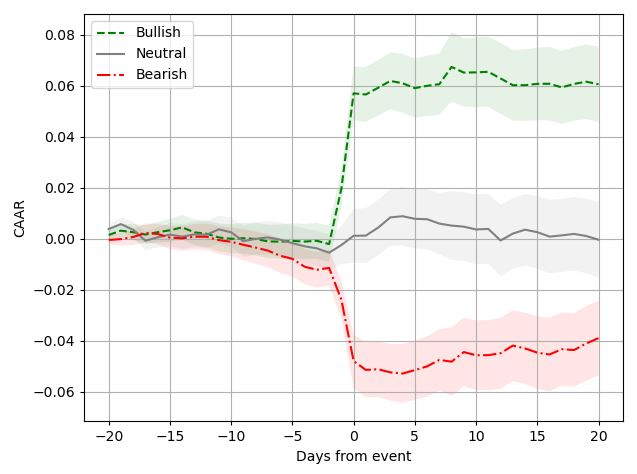
\includegraphics[width=0.5\textwidth]{caar.JPG}
%    \caption{Cumulative average abnormal returns around identified events. CAAR related to bearish, neutral and bullish events are displayed with the red, gray and green line, respectively. Areas around lines show confidence intervals at the 95\% level.}
%    \label{fig:ES_CAAR_MM}
%\end{figure}

%\clearpage
\subsection{Abnormal Polarity}
How does sentiment polarity behave around events? Similar to the above, we use as benchmark model a one-year rolling window regression of the daily polarity of ticker $i$ on the daily market polarity defined in \eqref{marketpoleq}, 
\begin{equation}
    P_{i,t}= \alpha_i^P  + \beta_i^P \cdot P_t^M  + \epsilon_{i,t},
\end{equation}
which gives the one-year rolling estimates $\hat{\alpha}_i^P$ and $\hat{\beta}_i^P$. This implies the abnormal polarity 
\begin{equation}
      AP_{i,t} = P_{i,t} - \left(\hat{\alpha_i}^P + \hat{\beta_i}^P \cdot P_t^M\right).
\end{equation}
We define the cumulative abnormal polarity (CAP) around a ticker $i$ event $\tau$ as 
\begin{equation}\label{eq_CAPtaut}
    CAP_i(\tau,t) = \sum_{s=- 20}^{t} AP_{i,\tau + s},
\end{equation}     
and the cumulative average abnormal polarities (CAAP) across all $N=1131$ events as 
\begin{equation}
       CAAP(t) = \dfrac{1}{N} \sum_{j=1}^N CAP_{i_j}(\tau_j,t).
\end{equation}

The right plot of Figure \ref{fig:caarcaap} shows the CAAP around the events. There are two main findings. First, in contrast to CAAR, the CAAP for bullish and bearish events is not constant after the event date, suggesting that users' sentiments about stocks tend to be biased towards recent past events. A possible explanation is that users might still post bullish (bearish) messages about a bullish (bearish) event during several days after the event. This is in contrast to the returns that immediately normalize after the event. Second, and more interestingly, the CAAP for bullish and bearish events shifts several days earlier than the CAAR. This indicates that investors are on average able to anticipate the type of an event in the near future. However, this sentiment only manifests through the social media, but not through abnormal returns. 

%\begin{figure}[h]
%    \centering
%    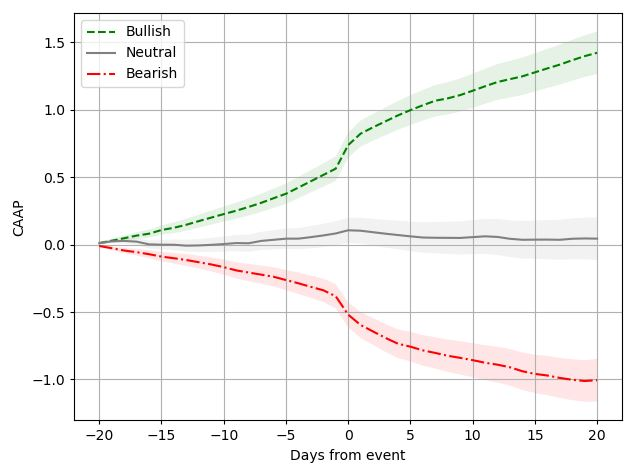
\includegraphics[width=0.5\textwidth]{caap.JPG}
%    \caption{Cumulative average abnormal polarity around identified events. CAAP related to bearish, neutral and bullish events are displayed with the red, gray and green line, respectively. Areas around lines show confidence intervals at the 95\% level.}
%    \label{fig:ES_cum_abn_pol_MM}
%\end{figure}

\begin{figure*}[h!]
\centering
        \begin{subfigure}{0.49\textwidth}   
            \centering 
            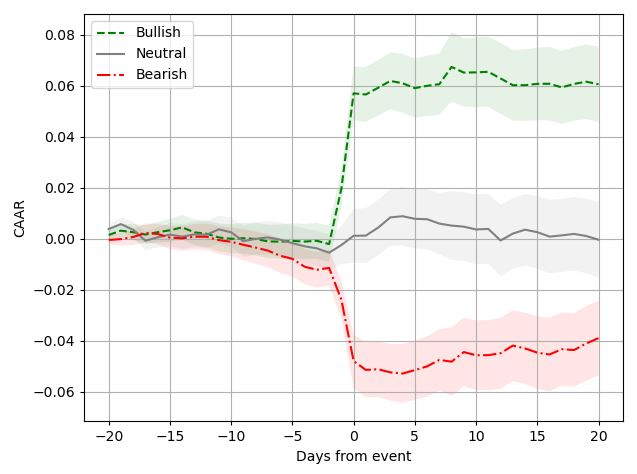
\includegraphics[width=\textwidth]{caar.jpg}
        \end{subfigure}
        \begin{subfigure}{0.49\textwidth}   
            \centering 
            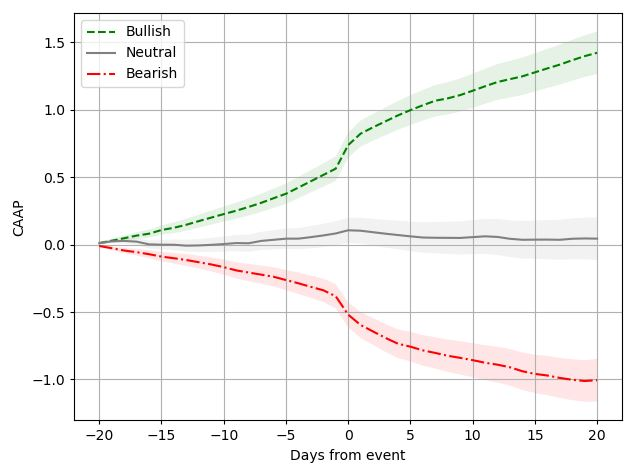
\includegraphics[width=\textwidth]{caap.jpg}
        \end{subfigure}
        \mycaption{CAAR and CAAP around identified events}{Cumulative average abnormal returns (left plot) and cumulative average abnormal polarity (right plot) around identified events. CAAR and CAAP related to bearish, neutral and bullish events are displayed with the red, gray and green line, respectively. Areas around lines show confidence intervals at the 95\% level.} 
        \label{fig:caarcaap}
\end{figure*}



Figure \ref{fig:boxplotcaar} illustrates this striking finding with box plots (see \citet{boxplot1} and \citet{boxplot2}) showing the distributions of the CAR and CAP, for all three event types, 5 days before the event, at the event date, and 5 days after the event, respectively. 

\begin{figure*}[h!]
        \centering
        \begin{subfigure}[b]{0.47\textwidth}
            \centering
            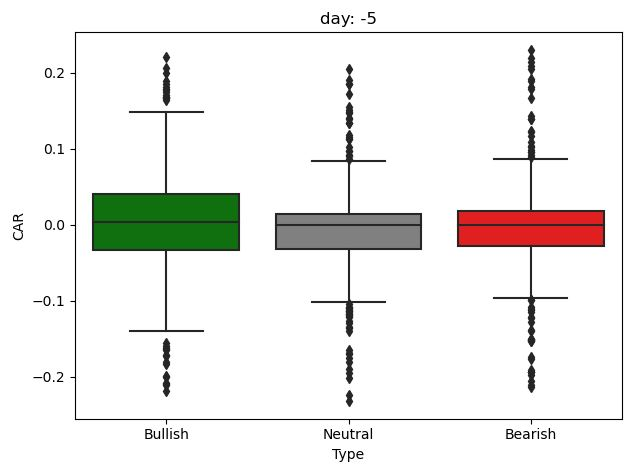
\includegraphics[width=\textwidth]{box_car_t-5.JPG}
            \caption*{CAR 5 days before the event}
        \end{subfigure}
        \quad
        \begin{subfigure}[b]{0.47\textwidth}  
            \centering 
            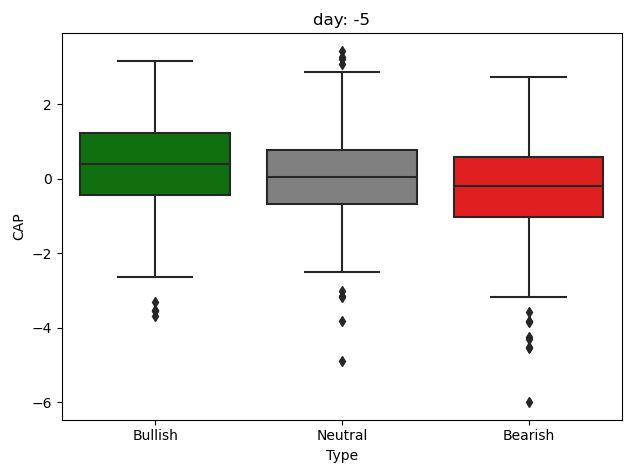
\includegraphics[width=\textwidth]{box_cap_t-5.JPG}
            \caption*{CAP 5 days before the event}  
        \end{subfigure}
        \vskip\baselineskip
        \begin{subfigure}[b]{0.47\textwidth}   
            \centering 
            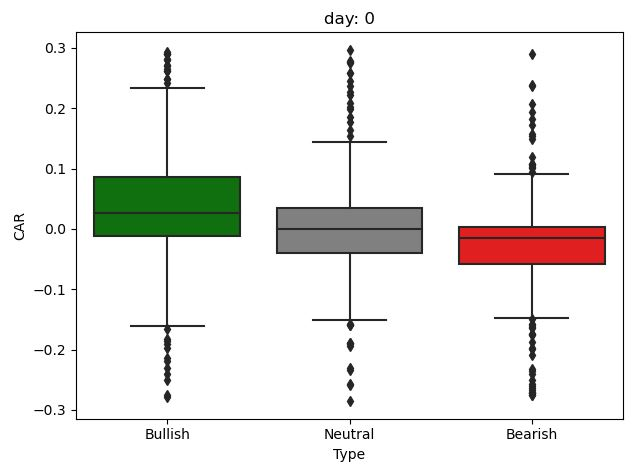
\includegraphics[width=\textwidth]{box_car_t.JPG}
            \caption*{CAR on the event date}   
        \end{subfigure}
        \quad
        \begin{subfigure}[b]{0.47\textwidth}   
            \centering 
            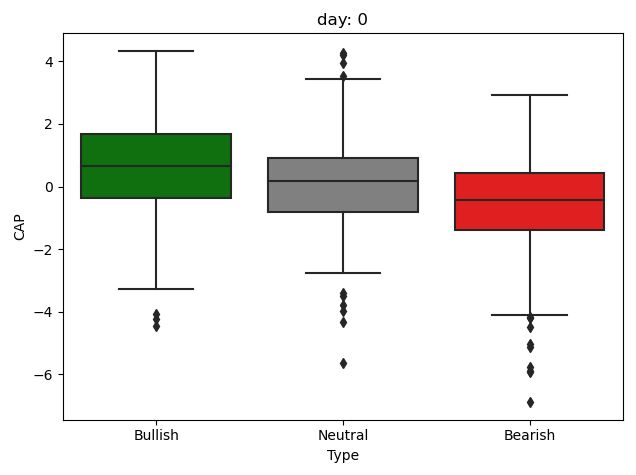
\includegraphics[width=\textwidth]{box_cap_t.JPG}
            \caption*{CAP on the event date}   
        \end{subfigure}
                \vskip\baselineskip
        \begin{subfigure}[b]{0.47\textwidth}   
            \centering 
            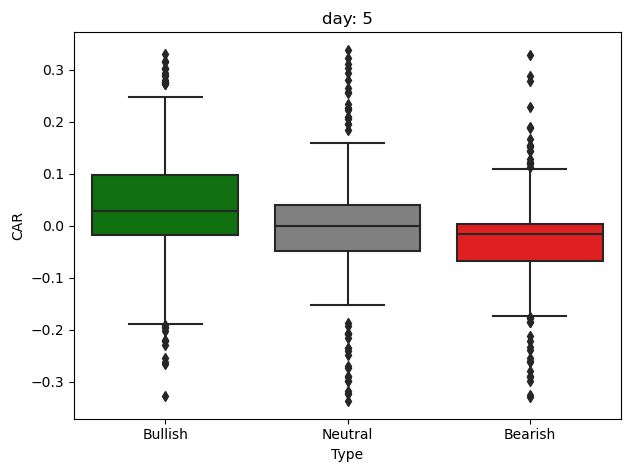
\includegraphics[width=\textwidth]{box_car_t+5.JPG}
            \caption*{CAR 5 days after the event}
        \end{subfigure}
        \quad
        \begin{subfigure}[b]{0.47\textwidth}   
            \centering 
            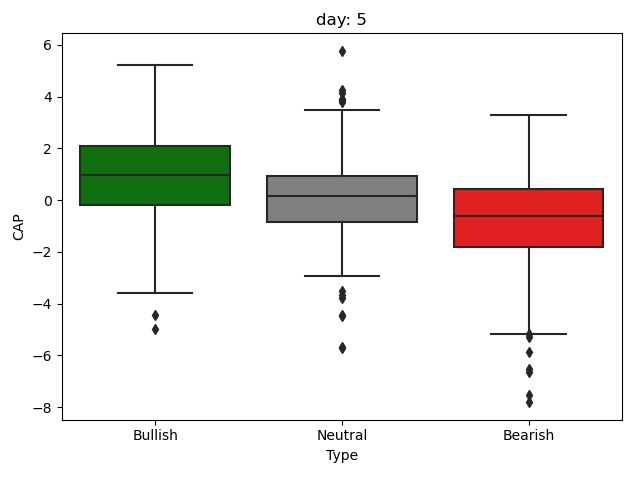
\includegraphics[width=\textwidth]{box_cap_t+5.JPG}
            \caption*{CAP 5 days after the event}  
        \end{subfigure}
        \mycaption{Distributions of CAP and CAR around events}{The line inside a box shows the median while the edges of each box represent the 25\% and 75\% quantile of the distribution. From above the edges of a box, a distance of 1.5 times the interquartile range is measured and a whisker is drawn up to the largest and lowest observed point from the data that falls within this distance. Interquartile range is equal to the third quartile minus the first quartile.} 
        \label{fig:boxplotcaar}
    \end{figure*}

\clearpage
To check statistical significance, we use the Mann-Whitney U-test (see \citet{utest} and \citet{sheskin}) to test whether the three samples (bullish, neutral and bearish) represent populations with different median values.\footnote{This interpretation only holds under stringent assumptions on the populations, namely that the two population distributions are equal up to a shift. Under the null hypothesis, the three samples represent distributions with equal medians. Let $\theta_i$ be the median of the distribution i. Formally, we test $H_0 : \theta_{bullish} = \theta_{neutral}$ against $H_1 : \theta_{bullish} > \theta_{neutral}$ and $H_0 : \theta_{neutral} = \theta_{bearish}$ against $H_1 : \theta_{neutral} > \theta_{bearish}$ 5 days before an event, on event date and 5 days after an event. We define U as the Mann-Whitney test statistic, Z as the normal approximation of the Mann-Whitney test statistic for large sample sizes, $n_1$ and $n_2$ as the sample sizes. We refer to \citet{sheskin} for the test statistic computation.}
Table \ref{utest_res} shows U-test statistics for pairwise comparisons. The null is rejected in every case except for CAR at $\tau-5$. That is, 5 days before the event, CAR has no predictive power on the type of event. This is consistent with the EMH. In contrast, 5 days before the event, CAP can predict the type of event. At the event date, the medians of the CAR shift as the abnormal returns jump for both bullish and bearish events. This is also consistent with the EMH. Finally, 5 days after the event, the distributions of the CAR are very similar to the ones at the event date. Again, this is consistent with the EMH, as all new information is instantaneously embedded into the prices and the returns normalize after the event, immediately. The medians of the CAP 5 days after the event exhibit an extended shift compared to the ones at the event date, as investors continue to post about recent past events.






% Please add the following required packages to your document preamble:
% \usepackage{multirow}
\begin{table} 
\centering
\begin{tabular}{|c|c|c|c|c|c|}
\hline
\multicolumn{6}{|c|}{CAR}                                                                                                                                    \\ \hline 
\multicolumn{1}{|l|}{}                     & Alternative Hypothesis                                                         & U     & Z        & $n_1$ & $n_2$ \\ \hline
\multicolumn{1}{|l|}{\multirow{2}{*}{$\tau$-5}} & $H_1$ : $\theta_{bullish} > \theta_{neutral}$ & 61109 & -1.70    & 452  & 292  \\
\multicolumn{1}{|l|}{}                     & $H_1$ : $\theta_{neutral} > \theta_{bearish}$  & 54168 & -0.52    & 292  & 380  \\ \hline
\multirow{2}{*}{$\tau$}                         & $H_1$ : $\theta_{bullish} > \theta_{neutral}$ & 50967 & -5.25*** & 452  & 292  \\
                                           & $H_1$ : $\theta_{neutral} > \theta_{bearish}$  & 43100 & -4.96*** & 292  & 380  \\ \hline
\multirow{2}{*}{$\tau$+5}                       & $H_1$ : $\theta_{bullish} > \theta_{neutral}$ & 52738 & -4.63*** & 452  & 292  \\
                                           & $H_1$ : $\theta_{neutral} > \theta_{bearish}$  & 43239 & -4.91*** & 292  & 380  \\ \hline \hline
\multicolumn{6}{|c|}{CAP}                                                                                                                                    \\ \hline
\multicolumn{1}{|l|}{}                     & Alternative Hypothesis                                                         & U     & Z        & $n_1$ & $n_2$ \\ \hline
\multicolumn{1}{|l|}{\multirow{2}{*}{$\tau$-5}} & $H_1$ : $\theta_{bullish} > \theta_{neutral}$ & 55408 & -3.70*** & 452  & 292  \\
\multicolumn{1}{|l|}{}                     & $H_1$ : $\theta_{neutral} > \theta_{bearish}$  & 47998 & -3.00***   & 292  & 380  \\ \hline
\multirow{2}{*}{$\tau$}                         & $H_1$ : $\theta_{bullish} > \theta_{neutral}$ & 49385 & -8.98*** & 452  & 292  \\
                                           & $H_1$ : $\theta_{neutral} > \theta_{bearish}$  & 42101 & -5.36*** & 292  & 380  \\ \hline
\multirow{2}{*}{$\tau$+5}                       & $H_1$ : $\theta_{bullish} > \theta_{neutral}$ & 44364 & -7.55*** & 452  & 292  \\
                                           & $H_1$ : $\theta_{neutral} > \theta_{bearish}$  & 40515 & -6.00*** & 292  & 380  \\ \hline
\end{tabular}
\mycaption{Mann-Whitney U-test statistics}{Mann-Whitney U-test statistics for pairwise significant differences between distribution medians. Under the null hypothesis, the two samples represent two distributions with equal median values. Statistical significance at the 99\%, 95\%, and 90\% level is indicated with ***, **, *, respectively.}
\label{utest_res}
\end{table}

\clearpage\section{Sentiment-Sorted Portfolios} \label{S:portfolios}

We assess the economic relevance of the sentiment polarity and construct sorted portfolios. Thereto, we define for every ticker $i$ and day $t$ 
\begin{equation}
     CAP_{i,t}=\sum_{s=t-14}^t AP_{i,s},
\end{equation}
which is the running CAP over the last 14 days plus the current day $t$ (we rebalance the portfolio at the close on day $t$).\footnote{As above, we work here with the restricted sample of 19 tickers and dates $t$ ranging through all business days of the sample period, excluding the first 14 days (for the CAP) and the last day (for the last portfolio holding period).} Note the difference to \eqref{eq_CAPtaut}. While we cannot predict the arrival of an event, we assume that the more $CAP_{i,t}$ deviates from zero the more likely there will be an event on the next day. We will thus use $CAP_{i,t}$ as a baseline signal for market timing. However, as we have seen above, CAP continues to shift after an event. To avoid exposures to short-term reversals, we thus reset the running CAP after every event. Formally, let $\tau_{i,t}\le t$ denote the most recent past event date by $t$ of ticker $i$. Then we define the reset CAP
\begin{equation}
    CAP_{i,t}^{(R)} = \sum_{s=\max\{t-14,\tau_{i,t}+1\}}^t AP_{i,s} = \begin{cases} CAP_{i,t},&\text{if $\tau_{i,t}<t-14$,} \\ \sum_{s= \tau_{i,t}+1}^t AP_{i,s},&\text{if $t-14\le \tau_{i,t}<t$,}\\
0,&\text{if $\tau_{i,t}=t$,}\end{cases}
\end{equation}
where we used the convention that $\sum_{s=t+1}^t \cdot =0$.

We also define time-varying thresholds on the reset CAP for market timing. For every day $t$, we estimate the mean $\mu_t$ and standard deviation $\sigma_t$ of $CAP_{i,t}^{(R)}$ across the 19 tickers $i$. For a fixed multiplier $x$, we define $U_t(x) = \mu_t + x \cdot \sigma_t$ the upper threshold, and $L_t(x) = \mu_t - x \cdot \sigma_t$ the lower threshold. Figure \ref{fig:cross-sec stats} shows the time series of the cross-sectional mean $\mu_t$ and the 99\% confidence interval, $L_t(x)$ and $U_t(x)$ for $x = 2.58$. As a robustness check of our approach, we observe that the mean is well centered at zero. We also see a regime change in early 2015. In the first regime the standard deviation is much larger (and more volatile) than in the second regime.\footnote{We could not find an exogenous cause for this regime change.} Appendix~\ref{app_CAPport} contains the results for the 95\% ($x = 1.96$) and 99.5\% ($x = 2.81$) confidence intervals. 

\begin{figure}[h]
    \centering
    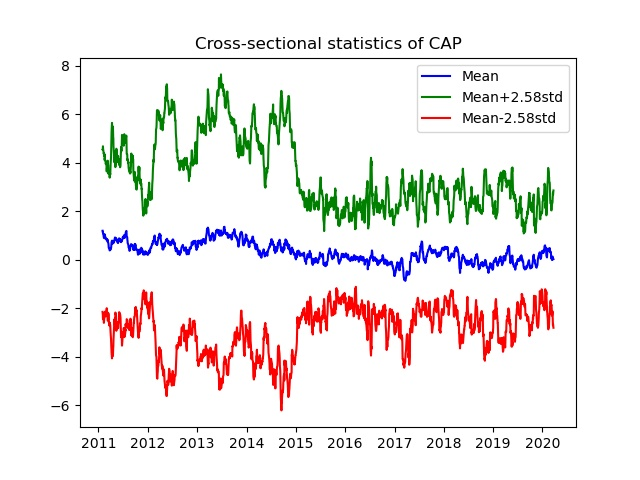
\includegraphics[width=0.75\textwidth]{cross_sectional_cap.jpg}
    \mycaption{Cross-sectional statistics of $CAP_{i,t}^{(R)}$}{The blue line shows the daily cross-sectional mean, the green (red) line shows the cross-sectional mean plus (minus) 2.58 standard deviations, respectively.}
    \label{fig:cross-sec stats}
\end{figure}

Based on these signals, we now construct reset-CAP-sorted portfolios. Formally, we define the ticker sets $I^{bull}_t=\{ i\mid CAP_{i,t}^{(R)} > U_t(x)\}$ and $I^{bear}_t=\{ i\mid CAP_{i,t}^{(R)} < L_t(x)\}$. At the close of any day $t$, we form the equally weighted bullish (bearish) portfolio consisting of tickers in $I^{bull}_t$ (in $I^{bear}_t$), and realize the 1-day returns. If any of the index sets is empty, we set the corresponding return to zero. The top-left plot of Figure \ref{fig:pf} shows the cumulative log returns of bullish and bearish portfolios as well as the S\&P500. Overall, the portfolio performance is consistent with our approach: the bullish (bearish) portfolio outperforms (under-performs) the market. Remarkably, the upward (downward) steps suggest that our portfolio strategy succeeds to take the right positions just before an event. The remaining plots of Figure \ref{fig:pf} show the number of positions across time of our portfolios. Most of the returns are earned with portfolios consisting of very few tickers. This is a result of our market timing and stock picking strategy: we only invest in the top/bottom percentiles of CAP, whenever our signal is strong enough.


% \begin{figure*}[h]
% \centering
% \begin{subfigure}{0.5\textwidth}  
%             \centering 
%             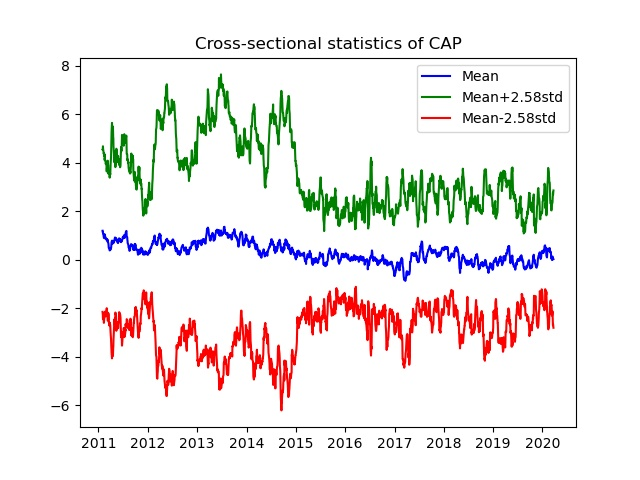
\includegraphics[width=\textwidth]{cross_sectional_cap.jpg}
%         \end{subfigure}
%         \quad
%         \begin{subfigure}{0.5\textwidth}   
%             \centering 
%             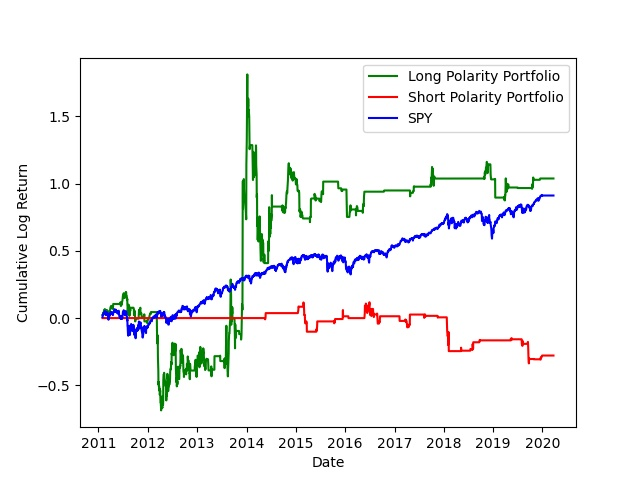
\includegraphics[width=\textwidth]{cumulative_log_return.jpg}
%         \end{subfigure}
%         \caption{Top graph shows the cross-sectional statistics of $CAP_{i,t}^{(R)}$. The blue lines shows the cross-sectional mean of the reset CAP across the 19 tickers over the year. The green and red lines show the up and down 99\% confidence band. We use them as up and lower thresholds for the portfolio construction. Bottom graph shows the cumulative log returns of bullish and bearish portfolios for $x =2.58$, and S\&P500.} 
%         \label{fig:pfconstruction258}
% \end{figure*}



%\begin{figure}[h!]
%    \centering
%    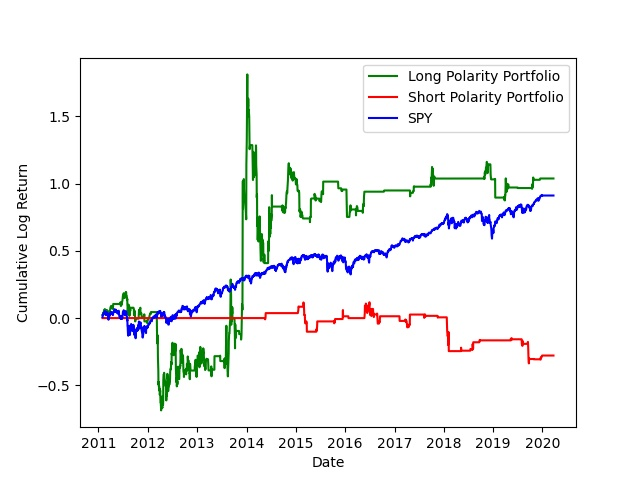
\includegraphics[width=0.5\textwidth]{cumulative_log_return.jpg}
%    \caption{Cumulative log returns of bullish and bearish portfolios for $x =2.58$, and S\&P500.}
%    \label{fig:cumretpf}
%\end{figure}




\begin{figure*}[h]
        \centering
        %\begin{subfigure}[b]{0.42\textwidth}
        %    \centering
        %    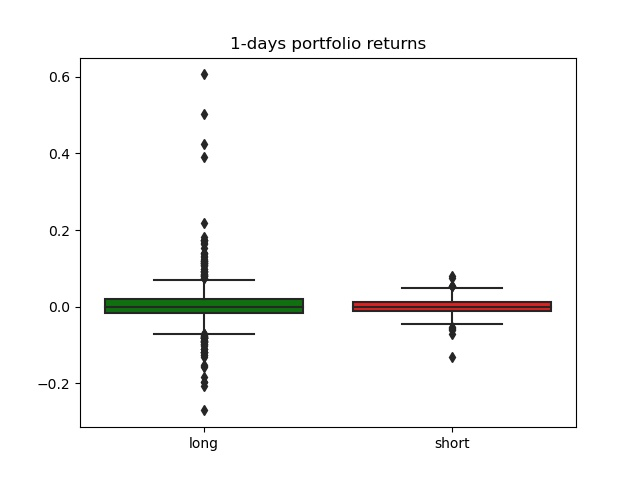
\includegraphics[width=\textwidth]{boxplot.JPG%}
        %    \caption*{Distribution of returns}
        %\end{subfigure}
        %\quad
        %\begin{subfigure}[b]{0.42\textwidth}  
        %    \centering 
        %    \includegraphics[width=\textwidth]{boxplot_zoo%med.JPG}
        %    \caption*{Distribution of returns - zoomed}  
        %\end{subfigure}
        %\vskip\baselineskip
        \begin{subfigure}[b]{0.42\textwidth}   
            \centering 
            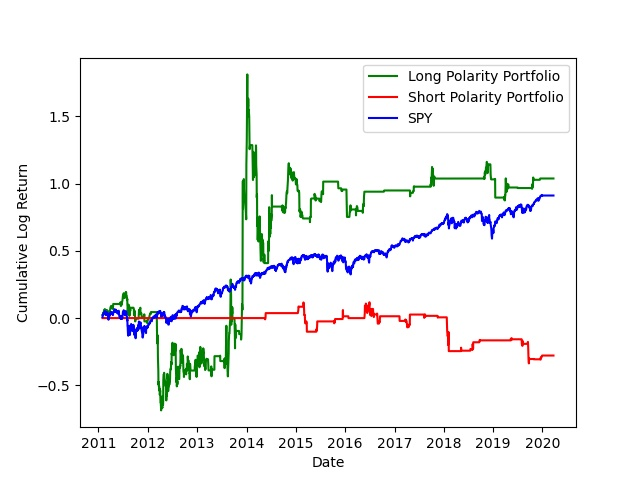
\includegraphics[width=\textwidth]{cumulative_log_return.jpg}
            \caption*{Cumulative log returns}
        \end{subfigure}
        \quad
        \begin{subfigure}[b]{0.42\textwidth}   
            \centering 
            \includegraphics[width=\textwidth]{distribution_positions.JPG}
            \caption*{Distribution of number of positions}   
        \end{subfigure}
                \vskip\baselineskip
        \begin{subfigure}[b]{0.42\textwidth}   
            \centering 
            \includegraphics[width=\textwidth]{positions.JPG}
            \caption*{Number of positions over time}
        \end{subfigure}
        \quad
        \begin{subfigure}[b]{0.42\textwidth}   
            \centering 
            \includegraphics[width=\textwidth]{returns.JPG}
            \caption*{Daily returns}  
        \end{subfigure}
        \mycaption{Bullish and bearish portfolios for $x=2.58$}{Top left plot shows the cumulative log returns of the portfolios over the years, top right plot shows the distribution of the number of positions in the portfolios, bottom left plot is the number of positions over time and bottom right plot is the daily returns of both portfolios.}
        \label{fig:pf}
    \end{figure*}




%\input{drawdowns}
\clearpage
\section{Conclusion} \label{S:conclusion}

We extract a large sample of messages from StockTwits from January 2010 to March 2020, covering US and Canadian stocks. Messages are either user-labeled as bullish or bearish or left unlabeled. Using the user-labeled messages as training set, we run logistic regressions on TFIDF vectorized messages to classify all unlabeled messages as either bullish, neutral or bearish. We observe a 5-to-1 bullish-to-bearish ratio, indicating that investors are on average optimistic. We build time series of daily sentiment polarity for individual tickers and the aggregate market. We show that daily polarity is positively associated to contemporaneous stock returns, but this result loses its significance against next-day returns. We then define events as days with sudden peaks of message volume and relate them to corporate and stock market events. We show that cumulative abnormal polarity has significant predictive power on the type of event, in contrast to cumulative abnormal returns. We also note that investor sentiment about a ticker tends to be biased towards recent past events. As robustness check, we show that our event study on cumulative abnormal returns is consistent with previous literature on the efficient market hypothesis. The performance of sentiment-sorted portfolios illustrates the economic relevance of our sentiment measure.
